\documentclass[12pt,a4paper]{article}
\usepackage[utf8]{inputenc}
\usepackage{amsmath}
%\usepackage[brazilian]{babel} % Brazil or not Brazil??
\usepackage{amsfonts}
\usepackage{amssymb}
\usepackage{graphicx}

\usepackage[margin=0.8in]{geometry}


\begin{document}
\title{\vspace{70mm}\Huge Experimento 06b - Calorimetria}
\author{ Giovani Garuffi\qquad\hfill
		\textit {RA: 155559}\protect\\
		João Baraldi\hfill
		\textit{RA: 158044}\protect\\
		Lauro Cruz\hfill
		\textit{RA: 156175}\protect\\
		Lucas Schanner\hfill
		\textit{RA: 156412}\protect\\
		Pedro Stringhini\hfill
		\textit {RA: 156983}								
		}
\maketitle
\newpage
\section{Resumo}

\section{Objetivos}
Este experimento pode ser divido em duas partes, cada uma com seus objetivos, que são: a determinação do calor específico de três metais diferentes (acreditados de serem chumbo, alumínio e cobre), e a determinação do calor latente de fusão do gelo. 


\section{Procedimento Experimental e Coleta de Dados}


\subsection{Procedimento}


\subsubsection{Determinação do Calor Específico de Metais}

Esta parte do experimento foi feita da seguinte maneira: com um ebulidor, aquece-se uma amostra de água, numa garrafa térmica, e imerge-se a amostra do metal, de massa obtida com uma balança($m_{metal}$), nessa água, mantendo-se o controle de sua temperatura com um termômetro de mercúrio ($\theta_{quente}$). Então, insere-se o metal aquecido no calorímetro com água fria (vide figura \ref{CalorMetais}), de temperatura ($\theta_{frio}$) e massa ($m_{H_2O}$) também conhecidos, e espera-se pelo equilíbrio térmico ($\theta_{final}$), para anotar seu valor.

\begin{figure}[!htbp]
\centering
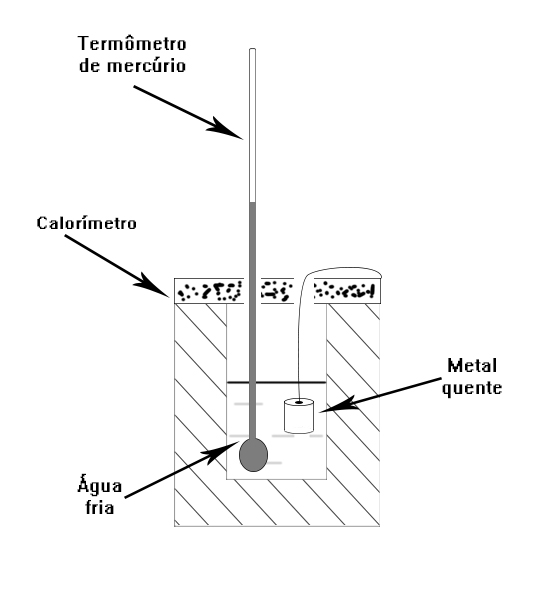
\includegraphics[scale=0.45]{Fig6b1.jpg}
\caption{Exemplo da montagem experimental da primeira parte do experimento.}
\label{CalorMetais}
\end{figure}

Assim, calcula-se o calor específico do metal através da seguinte forma:

$$\Sigma Q = 0$$\
$$Q_{cedido\; pelo\; metal} + Q_{recebido\; por\; H_2O} + Q_{recebido\; pelo\; calorimetro} = 0$$\
$$m_{metal} \; c_{metal} \; (\theta_{final} - \theta_{quente}) + m_{H_2O} \; c_{H_20} \;  (\theta_{final} - \theta_{frio}) + C_{calorimetro} \; (\theta_{final} - \theta_{frio}) = 0$$\
$$c_{metal} = \frac{m_{H_2O} \; c_{H_20} \;  (\theta_{final} - \theta_{frio}) + C_{calorimetro} \; (\theta_{final} - \theta_{frio})}{m_{metal} \;(\theta_{quente} - \theta_{final})}$$\

Então, repete-se o procedimento para as demais amostras.

\subsubsection{Determinação do Calor Latente de Fusão do Gelo}

Esta outra parte é feita de forma análoga. Insere-se uma massa $m_{gelo}$ (encontrado com a balança) de gelo, de temperatura conhecida ($\theta_{fusao}$), no calorímetro preenchido até a metade com água fria, de massa ($m_{agua}$) e temperatura ($\theta_{agua}$) conhcidos, até atingir-se o equilíbrio térmico ($\theta_{equilibrio}$), medindo-se seu valor com o termômetro, como mostrado na figura \ref{CalorGelo}.

\begin{figure}[!htbp]
\centering
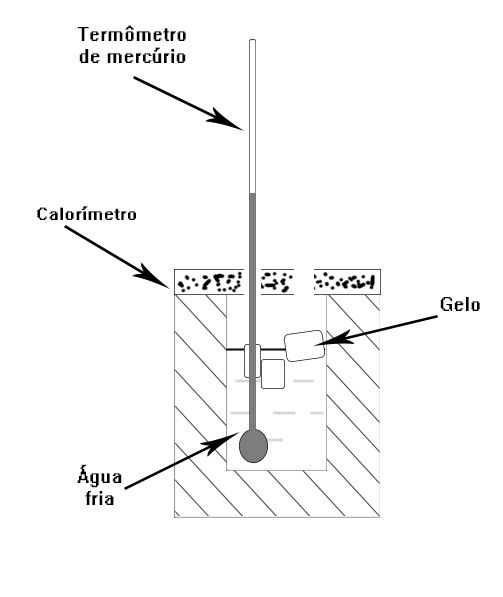
\includegraphics[scale=0.45]{Fig6b2.jpg}
\caption{Exemplo de montagem experimental da segunda parte do experimento.}
\label{CalorGelo}
\end{figure}

Então, pelo mesmo princípio do item anterior, considerando o aquecimento da massa de gelo, após seu derretimento, e assumindo que o gelo estava em fusão desde o inicio, temos:

$$Q_{recebido\;pelo\;gelo} + Q_{cedido\;pela\;agua} + Q_{cedido\;pelo\;calorimetro} = 0$$\
$$m_{gelo} \; L_{fusao\;do\;gelo} \; + \; m_{gelo} \; c_{agua} \; (\theta_{equilibrio} - \theta_{fusao}) \; + \; m_{agua} \; c_{agua} \; (\theta_{equilibrio} - \theta_{agua}) \;$$ $$+ \; C_{calorimetro} \; (\theta_{equilibrio} - \theta_{agua}) = 0$$\
$$L_{fusao\;do\;gelo} = \frac{1}{m_{gelo}} \cdot (m_{gelo} \; c_{agua} \; (\theta_{fusao} - \theta_{equilibrio}) \; + \; m_{agua} \; c_{agua} \; (\theta_{agua} - \theta_{equilibrio}) \;$$ 
$$ + \; C_{calorimetro} \; (\theta_{agua} - \theta_{equilibrio}))$$


\subsection{Dados Obtidos}

%ficou feio esse primeiro paragrafo não-identado... Se quiser mudar tem uma \usepackage{indentfirst} que é sucesso.
Para o chumbo, obtivemos os seguintes valores:
$$ T_{quente} = (75,0 \pm 0,5)\,^{\circ}\mathrm{C}, \qquad T_{frio} = (22,0 \pm 0,5)\,^{\circ}\mathrm{C}, $$
$$ m_{Metal} = (102,0 \pm 0,5)g, \qquad T_{equilibrio} = (23,0 \pm 0,5)\,^{\circ}\mathrm{C}. $$


Para o alumínio, obtivemos os seguintes valores:
$$ T_{quente} = (72,5 \pm 0,5)\,^{\circ}\mathrm{C}, \qquad T_{frio} = (24,0 \pm 0,5)\,^{\circ}\mathrm{C}, $$
$$ m_{Metal} = (42,3 \pm 0,1)g, \qquad T_{equilibrio} = (26,0 \pm 0,5)\,^{\circ}\mathrm{C}. $$


 E finalmente, para o cobre, temos:
$$ T_{quente} = (67,0 \pm 0,5)\,^{\circ}\mathrm{C}, \qquad T_{frio} = (26,5 \pm 0,5)\,^{\circ}\mathrm{C}, $$
$$ m_{Metal} = (91,6 \pm 0,1)g, \qquad T_{equilibrio} = (27,5 \pm 0,5)\,^{\circ}\mathrm{C}. $$

A Massa de água à temperatura ambiente utilizada em cada um dos experimentos é $185.7 \pm 0.1 \; g$.


\section{Análise dos Resultados e Discussões}

\subsection{Determinação do Calor Específico de Metais}
Da formula 
$$c_{metal} = \frac{m_{H_2O} \; c_{H_20} \;  (\theta_{final} - \theta_{frio}) + C_{calorimetro} \; (\theta_{final} - \theta_{frio})}{m_{metal} \;(\theta_{quente} - \theta_{final})}$$\

Obtemos 
$$ c_{chumbo} = 0.042552 $$
$$ c_{aluminio} = 0.22949 $$
$$ c_{cobre} = 0.062379 $$

Propagando o erro, obtemos a formula 
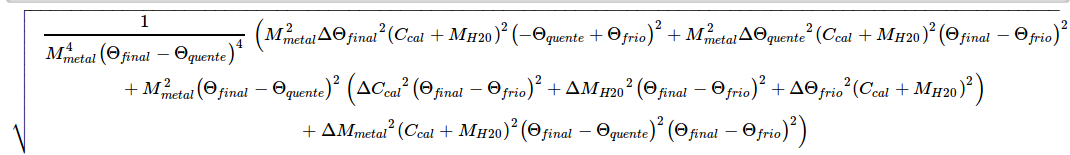
\includegraphics[scale=1]{formula.png}

$$ \Delta c_{chumbo} = 0.03 $$
$$ \Delta c_{aluminio} = 0.09 $$
$$ \Delta c_{cobre} = 0.05 $$

Então os valores finais podem ser escritos como 
$$ c_{chumbo} = 0.04 \pm 0.03 \; cal/gC$$
$$ c_{aluminio} = 0.23 \pm 0.09 \; cal/gC$$
$$ c_{cobre} = 0.06 \pm 0.05 \; cal/gC$$

\subsection{Determinação do Calor Latente de Fusão do Gelo}


\section{Conclusões}

\end{document}

